% Numerical Computing II
% Homework 19
% Eigenvalues, ODE's, and Control
% 3/20/2010
% 19.1, 19.2,19.3,19.4,19.5,19.7,19.8(use matlab)
% 19.9, 19.10,19.12.19.14,19.17-19

\documentclass[11pt]{article}
\usepackage{listings}
\usepackage{amsfonts}
\usepackage{amsthm}
\usepackage{verbatim}
\usepackage[fleqn]{amsmath}
\usepackage{graphicx}
\begin{document}         
% Start your text
\newcommand{\makehomework}[2]%
{\begin{center}%
	\Huge #1\\%
	\Large #2\\%
	Marty Fuhry\\%
	\today%
\end{center}}
\makehomework{Numerical Computing II}{Eigenvalues, ODE's, and Control}

\lstset{language=Matlab,numbers=left,frame=single,breaklines=true,morecomment=[l]{//}}
\section*{Exercise 19.1}
Since A is an upper triangular matrix, we can simply
pull the eigenvalues off the diagonal. Then, the 
characteristic polynomial is
\begin{align*}
    p_A(z) = (1 - z)(2 - z)(3 - z).
\end{align*}

\section*{Exercise 19.2}
A is not upper triangular, so we need to solve
\begin{flalign*}
    p_A(z) &= det(A - zI)\\
           &= \left|\begin{array}{ccc}
              0.5 - z & 1     & 1\\
              1       & 2 - z & 3\\
              0       & 0     & 3 - z\\
              \end{array}\right|\\
           &= (.5 - z)(2-z)(3-z) - (3-z). 
\end{flalign*}
\pagebreak
\section*{Exercise 19.3}
Using
\begin{flalign*}
    AV &= VD\\
    A  &= VDV^{-1},
\end{flalign*}
we can write $A^2$ as
\begin{flalign*}
    A^2 &= {(VDV^{-1})}^2\\
        &= (VDV^{-1})(VDV^{-1}).
\end{flalign*}
Recognizing that since $VV^{-1}= I$, we can simplify this expression as
\begin{flalign*}
    A^2 &= (VDV^{-1})(VDV^{-1})\\
        &= (VD)(V^{-1}V)(DV^{-1})\\
        &= (VD)(DV)\\
        &= VD^2V.
\end{flalign*}

In general, $A^k = VD^kV$ when $k \in \mathbb{N}$.

Then, when $k \in \mathbb{Z}$ and $k < 0$, and $A$ is nonsingular,
then $A^{-1}$ exists, and we can say,
\begin{flalign*}
    A^{-1}&= (VDV^{-1})^{-1}\\
         &= VD^{-1}V^{-1}\\
    (A^{-1})^k &= (VD^{-1}V^{-1})^k\\
     A^{-k}    &= VD^{-k}V^{-1}.
\end{flalign*}

\section*{Exercise 19.4}
We'll again use the spectral factorization of $A$:
\begin{flalign*}
    A &= VDV^{-1}
\end{flalign*}
The main question here is, "Does $A^{1/2} = VD^{1/2}V^{-1}?$" Let's start by 
defining the $n$ x $n$ matrix $M$ such that $A = MM$. Then,
\begin{flalign*}
    Ax &= \lambda x\\
    MMx &= \lambda x.
\end{flalign*}
So $A$ and $MM$ have the same eigenvalues and eigenvectors. That means,
\begin{flalign*}
    M &= \hat{V}\hat{D}\hat{V}^{-1}\\
    MM &= \hat{V}\hat{D}^2\hat{V}^{-1} = VDV^{-1} = A.
\end{flalign*}
Since $MM$ and $A$ have the same eigenvectors and eigenvalues, then $\hat{V} = V$ 
and $\hat{D}^2 = D$. This means, $MM = VDV^{-1}$. Now, to reduce this equation to just
$M$, we need to consider only the expression $\hat{D}^2 = D$. Since $\hat{D}$ and $D$
are both diagonal matrices, we can simply allow $\hat{D} = D^{1/2}$ and take the
square root of each entry of $D$ to form $\hat{D}$. Then, we have
\begin{flalign*}
    MM &= V\hat{D}^2V^{-1}\\
    M  &= VD^{1/2}V^{-1}.
\end{flalign*}
And since $M = A^{1/2}$, we finish with $A^{1/2} = VD^{1/2}V^{-1}$.

\qedsymbol

\section*{Exercise 19.5}
Let $c$ be some scalar such that $c \in \mathbb{R}$ with $c \neq 0$. We'll start by using
the fact that 
\begin{flalign*}
    Av &= \lambda v.
\end{flalign*}
We can create any nonzero multiple of $v$ by simply multiplying it by $c$. Let 
$\hat{v}$ be a nonzero multiple of $v$. That is, let $\hat{v} = cv$  It necessarily
follows that
\begin{flalign*}
    Av    &= \lambda v\\
    cAv   &= c \lambda v\\
    A(cv) &= \lambda (cv)\\
    A\hat{v} &= \lambda \hat{v}.
\end{flalign*}
\qedsymbol

\pagebreak
\section*{Exercise 19.7}
If $A = $diag$[1,1,3]$, then we can pull the eigenvalues of $A$ off the diagonal
by using the characteristic equation $p_A(z) = (1-z)(1-z)(1-3)$. Then, to verify
that $\lambda = 1, 3$, we can show that det($A-\lambda I) = 0$). 

First, we'll verify that when $\lambda = 1$, det($A - \lambda I) = 0$).
\begin{align*}
    det(\left[\begin{array}{ccc}
    1 & 0 & 0\\
    0 & 1 & 0\\
    0 & 0 & 3
    \end{array}\right]
    -
    \left[ \begin{array}{ccc}
    1 & 0 & 0\\
    0 & 1 & 0\\
    0 & 0 & 1
    \end{array}\right])\\
    = det(\left[\begin{array}{ccc}
    0 & 0 & 0\\
    0 & 0 & 0\\
    0 & 0 & 2
    \end{array}\right])\\
    = 0.
\end{align*}

Next, let's verify that when $\lambda = 3$, det($A - \lambda I) = 0$.

\begin{align*}
    det(\left[\begin{array}{ccc}
    1 & 0 & 0\\
    0 & 1 & 0\\
    0 & 0 & 3
    \end{array}\right]
    -
    \left[ \begin{array}{ccc}
    3 & 0 & 0\\
    0 & 3 & 0\\
    0 & 0 & 3
    \end{array}\right])\\
    = det(\left[\begin{array}{ccc}
    -2 & 0 & 0\\
    0 & -2 & 0\\
    0 & 0  & 0
    \end{array}\right])\\
    = 0.
\end{align*}
\pagebreak
\section*{Exercise 19.8}
Again, this is an upper triangular matrix, so we can pull the eigenvalues off the 
diagonal. We see that $\lambda = 1.01, 1$. Using the eig() command from an Octave
shell, we can get corresponding eigenvectors from $A$:
\begin{flalign*}
    v_1 &= \left[ \begin{matrix}
          1\\
          0
          \end{matrix} \right]\\
    v_2 &= \left[ \begin{matrix}
          -0.999987500234370 \\
           0.004999937501172
           \end{matrix} \right]
\end{flalign*}
We can see that $v_1$ and $v_2$ are "nearly" linearly dependent, but they are, in fact, linearly independent.
We can also observe that had the matrix $A$ used the value $1$ instead of $1.01$, we would see 
linearly dependent $v_1$ and $v_2$. 

We also note that $v_1$ and $v_2$ are nearly perpendicular. Observe the graph of $v_1$ and $v_2$.
\begin{center}
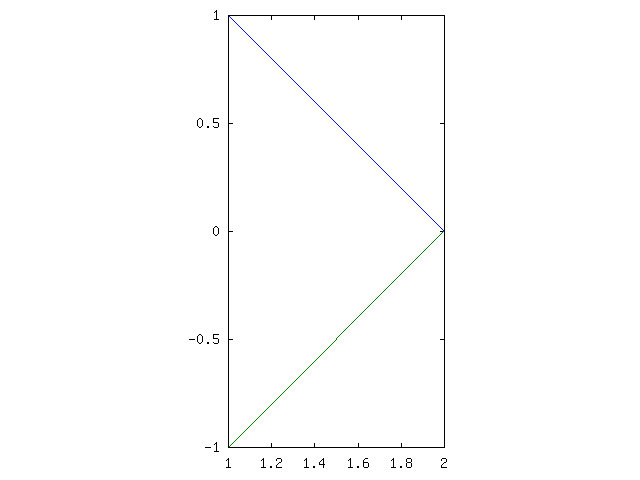
\includegraphics[scale=0.5]{problem_19_8.png}
\end{center}

Though, if we were to "negate" one of the eigenvectors, we would get a picture of nearly
parallel vectors. Let's see what happens when we multiply $v_2$ by $-1$.
\begin{center}
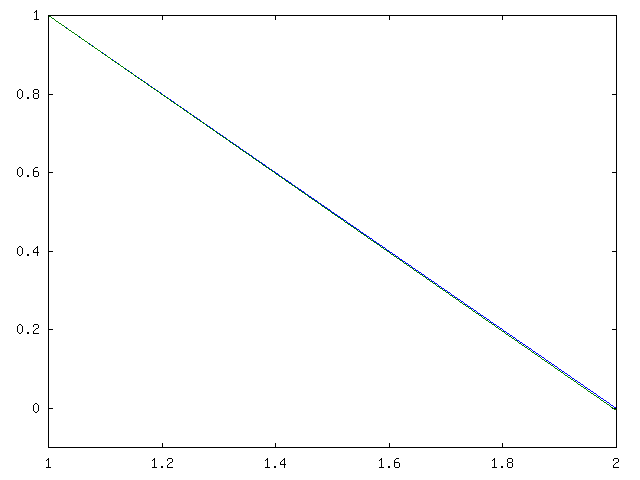
\includegraphics[scale=0.5]{problem_19_8_negate.png}
\end{center}

These are nearly on top of each other. However, if we were to examine very closely, we
would see them diverge ever so slightly. They are NOT parallel, but very nearly.

\section*{Exercise 19.9}
The magic matrix is shaped like:
\begin{align*}
    \left[ \begin{array}{cccc}
     16 &   2 &   3 &  13\\
     5  & 11 &  10  &  8\\
     9  &  7 &   6  & 12\\
     4  & 14 &  15  &  1
    \end{array} \right].
\end{align*}

Looking at the eigenvectors through the eig() command in Octave, we see
$\lambda = 34, \pm 8.94427, 0$. The only curious eigenvalue in the set
is $34$. We can add up each element of each row and obtain the value $34$.
Additionally, we can add up each element of each column and obtain the value
$34$. Clearly, $34$ has some significance in this problem.

Let's examine our eigenvectors. These correspond to 
$\lambda = 34, 8.94427, -8.94427, 0$ in that order.

\begin{flalign*}
    v_1 &= 
    &\left[ 
    \begin{array}{c}
    -.5\\
    -.5\\
    -.5\\
    -.5
    \end{array}
    \right]&
    , &v_2 = 
    &\left[ 
    \begin{array}{c}
    -0.823607\\
    0.423607\\
    0.023607\\
    0.376393
    \end{array}
    \right]&
    \\
     v_3 &= 
    &\left[
    \begin{array}{c}
     0.376393\\
     0.023607\\
     0.423607\\
    -0.823607
    \end{array}
    \right]&
    , &v_4 = 
    &\left[
    \begin{array}{c}
    -0.22361\\
    -0.67082\\
     0.67082\\
     0.22361
    \end{array}
    \right]&
\end{flalign*}

The eigenvector $v_1$, which corresponds to the eigenvalue
$\lambda = 34$ consists of identical entries. This is because of
the identical nature of each row and column adding up to become
the same number, which happens to be the $\lambda$ value corresponding
to this eigenvector.

The eigenvectors are all normalized to have a norm of 1. This is probably
because of Octave. The eigenvectors could have any discernable norm greater
than zero because there are infinite number of them. Octave just chose
to normalize them before returning them. Or perhaps this normalization is inherent in the
numerical method used to produce said eigenvectors. Regardless, the only
"important" eigenvalue to take away from this problem is probably $34$. 

\section*{Exercise 19.10}
The exp($n$) function in Octave will compute the value $e^{n}$.
The expm($A$) function in Octave will compute the exponential of a matrix $A$.
\begin{quote}
    \begin{verbatim}> help exp \end{verbatim}

    Compute the exponential of X.
\end{quote}
\begin{quote}
    \begin{verbatim}> help expm \end{verbatim}

    Return the exponential of a matrix, defined as the infinite Taylor
    series:

          expm($A$) $= I + a + a^2/2! + a^3/3! + \cdots $
\end{quote}
\emph{-From the Octave help command}

\section*{Exercise 19.12}
Solve $\displaystyle\max_{1\leq j \leq n} \{e^{\lambda_j t}\}$, where $\lambda_j < 0$, $ \forall j$. Choose $\lambda^{\star} = 
\displaystyle\min_{1 \leq j \leq n} \lambda_j$. We know $\lambda^{\star} < 0$ by hypothesis. 
\begin{align*}
    e^{\lambda^{\star} t} = \frac{1}{e^{-\lambda^{\star}t}}.
\end{align*}
Clearly, $-\lambda^{\star} \ge 0$. Then,
\begin{align*}
    \displaystyle\lim_{x\to\infty} \frac{1}{e^{-\lambda^{\star}t}} = 0.
\end{align*}
So, as $t$ increases without bound, $e^{\lambda^{\star}t}$ decreases to zero.

\qedsymbol

\section*{Exercise 19.14}
Using $\lambda = -1, -1, 0$, we can see that choosing $\lambda^{\star} =
\displaystyle\max_{1 \leq j \leq 3} {\lambda_j} = 0$. We then bound 
$||x||$ by $e^{\lambda^{\star} t} = e^0t = 1$, which does not depend on
$t$. $||x||$, then, may decrease due to do the other eigenvalues, but
will certainly not increase without bound, for it is bounded by a constant
value, which is $1$. At worst, it will stay constant or oscillate with bounded
amplitude $\forall t$. 

\section*{Exercise 19.17}
Since we've defined
\begin{flalign*}
    x(t) := \left[ \begin{array}{c}
        \hat{h}(t)\\
        \frac{d\hat{h}}{dt}(t)\\
        \hat{i}(t)
        \end{array}\right]
\end{flalign*}
we can derive
\begin{flalign*}
    \frac{d}{dt}x(t) := \left[ 
    \begin{array}{c}
        \frac{d}{dt}\hat{h}(t)\\
        \frac{d^2\hat{h}}{dt^2}(t)\\
        \frac{d}{dt}\hat{i}(t)
    \end{array}\right] .
\end{flalign*}
Then, we construct the system of equations which relate $\frac{d}{dt}x(t)$ to $x(t)$.
This has been done in the notes, so I'll just use
\begin{align*}
    A = \left[ \begin{array}{ccc}
        0 & 1 & 0\\
        1 & 0 & -1\\
        0 & 0 & -10
        \end{array}\right].
\end{align*}
We can solve for the eigenvalues of $A$ by using the eig() command in Octave, or
we can derive them quite simply from the characteristic equation 
\begin{flalign*}
    p_A(z) &= (-\lambda)(-\lambda)(-10 - \lambda) - (-10 - \lambda)\\
           &= -\lambda^3 -10\lambda^2 + \lambda + 10.
\end{flalign*}
Using Octave, we obtain eigenvectors $v_1, v_2, v_3$ corresponding to 
eigenvalues:
\begin{flalign*}
    \begin{array}{lll}
    \lambda_1 = -10, & \lambda_2 = -1, & \lambda_3 = 1\\
    v_1 = \left[ \begin{array}{c}
    -0.01005\\
    0.10049\\
    0.99489
    \end{array} \right], &
    v_2 = \left[ \begin{array}{c}
    -0.70711\\
    0.70711\\
    0
    \end{array} \right], &
    v_3 = \left[ \begin{array}{c}
    0.70711 \\
    0.70711 \\
    0
    \end{array} \right]. 
    \end{array}
\end{flalign*}
To solve our system of linear equations, we consider the solution to the homogenous
system of equations $\frac{d}{dt}x(t) = Ax(t)$. We recognize the solution $x(t) = \eta e^{rt}$ 
such that $\frac{d}{dt}x(t) = r\eta e^{rt}$, where $\eta$ is some vector of constants and 
$r$ is some constant. Then, we solve
\begin{flalign*}
    Ax(t) &= \frac{d}{dt}x(t)\\
    Ax(t) - \frac{d}{dt}x(t) &= 0\\
    A\eta e^{rt} - r \eta e^{rt} &= 0\\
    (A - rI)\eta e^{rt} &= 0.
\end{flalign*}
We see that solutions to this equation are clearly when $r$ is an eigenvalue
and $\eta$ is the corresponding eigenvalue of $A$. 

Since we know three seperate solutions to the equation $x(t)$:
\begin{flalign*}
    \begin{array}{ccc}
    x_1(t) &= \eta_1 e ^{r_1 t} &= \left[ \begin{array}{c}
    -0.01005\\
    0.10049\\
    0.99489
                                 \end{array} \right] e^{-10t}\\
    x_2(t) &= \eta_2 e ^{r_2 t} &= \left[ \begin{array}{c}
                                 -0.70711\\
                                 0.70711\\
                                 0
                                 \end{array} \right] e^{-t}\\
    x_3(t) &= \eta_3 e ^{r_3 t} &= \left[ \begin{array}{c}
                                 0.70711\\
                                 0.70711\\
                                 0
                                 \end{array} \right] e^t
    \end{array}
\end{flalign*}
Our general solution is obtained by adding each particular solution
and solving for the initial value $x_0$. We need to be sure the Wronskian
of these solutions is not zero.
\begin{flalign*}
    W[x_1, x_2, x_3](t) =& \left| 
        \begin{array}{ccc}
           0        & -0.70711 e^{-t} & 0.70711 e^t\\
           0        & 0.70711  e^{-t} & 0.70711 e^t\\
           e^{-10t} &   0             & 0
           \end{array} \right| \\
    =& (-0.70711 e^{-t}) (0.70711e^t)(e^{-10t}) \\&- (e^{-10t})(0.70711e^{-t})(0.70711e^t)\\
    =& -2e^{-10t}(0.70711)^2.
\end{flalign*}
$W[x_1, w_2, w_3](t)$ is never zero $\forall t$, so the solutions $x_1, x_2, x_3$ form a 
fundamental set of solutions. We'll use the method of undetermined coeffients to solve this
Assume $x(t)$ is of the form $x(t) = ae^{10t} + be^{-t} + ce^{t} + d$ where $a, b, c, $ and $d$ are
constants to be determined. Then, $\frac{d}{dt}x(t) = -10ae^{-10t} - be^{-t} + ce^{t}$.
\begin{flalign}
\label{sec:coeff}
    \frac{d}{dt} x(t) &= Ax(t)\\
    -10ae^{-10t} -be^{-t} +ce^{t} &= A(ae^{-10t}+be^{-t}+ce^{t} +d) + g
\end{flalign}
We then determine coefficient vectors $a, b, c, $and $d$ by matching up coefficients from
\ref{sec:coeff}.
\begin{flalign*}
    -10*a &= Aa\\
    -1*b &= Ab\\
     1*c &= Ac\\
       0 &= Ad + g
\end{flalign*}
Each of these solutions is the eigenvalue and eigenvector corresponding to the 
specific variables. Then $a = x_1$, $b = x_2$, $c = x_3$, and $Ad = -g$.

\begin{align*}
    Ad = -g\\
    \left[\begin{array}{ccc}
        0 & 1 & 0\\
        1 & 0 & -1\\
        0 & 0 & -10
    \end{array}\right] d =
    \left[\begin{array}{c}
        0\\
        1\\
        1
    \end{array}\right]
\end{align*}
We can solve for $d$ quite simply through Octave by the command 
\begin{verbatim}d = A\g \end{verbatim}.
\begin{align*}
    d = \left[\begin{array}{c}
        0.9\\
        0\\
        0.1
        \end{array}\right].
\end{align*}
The general solution is determined by adding together the fundamental set of solutions
with their appropriate coefficients.
\begin{flalign*}
    x(t) =& x_1 + x_2 + x_3 + d \\
         =& \left[ \begin{array}{c}
             -0.01005\\
              0.10049\\
              0.99489
              \end{array} \right] e^{-10t} + 
            \left[ \begin{array}{c}
              -0.70711\\
              0.70711\\
              0
            \end{array} \right] e^{-t} +
            \left[ \begin{array}{c}
              0.70711\\
              0.70711\\
              0
             \end{array} \right] e^t + 
            \left[ \begin{array}{c}
              0.9\\
              0\\
              0.1
             \end{array} \right].
\end{flalign*}
We can see that from our solutions, as $t$ grows without bound, 
$x_3 e^{t}$ will increase to infinity.

We should ook at the solution of $y(t)$, too, which is just
the first row of our solution $x(t)$.
\begin{align*}
    y(t) = -.01005*e^{-10t}-.70711*e{-t}+.70711*e^{t}+.9
\end{align*}

% Import Graph
\begin{center}
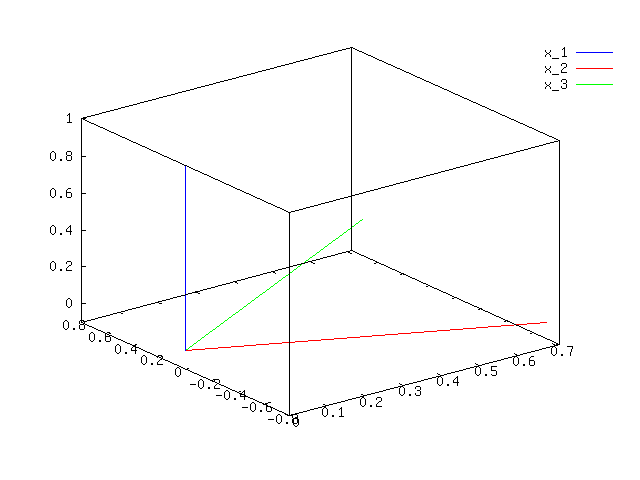
\includegraphics[scale=0.5]{problem_19_17.png}
\end{center}

We should be able to solve this a Numerical way, too. Namely,
\begin{flalign*}
    x(t) &= e^{At}x(0)\\
         &= (V e^D V^{-1})x(0)\\
         &= (\left[\begin{array}{ccc}
                v_1 &  v_2 & v_3
             \end{array}\right]
             \left[\begin{array}{ccc}
             e^{-10t} & 0 & 0\\
             0       & e^{-t} & 0\\
             0       & 0      & e^t
             \end{array}\right]
             \left[\begin{array}{ccc}
                v_1 & v_2 & v_3
             \end{array}\right]^{-1})x(0)
\end{flalign*}
This reduces to solving \begin{verbatim} x = V * expm(D) * V^-1\end{verbatim}.
Then, we line up our solution vectors, divide out the exponential terms
(since our numerical method solved for when $t = 1$, we divide out $e^a$
for the correct $a$ value. 
\begin{align*}
    x(t) = \left[\begin{array}{c}
        -0.037936\\
        -0.052971\\
        0.0000016
        \end{array}\right] e ^{-10t} + 
        \left[\begin{array}{c}
        3.1945\\
        4.1945\\
        0
        \end{array}\right] e ^{-t} + 
        \left[\begin{array}{c}
        33989\\
        25886\\
        0
        \end{array}\right] e ^t +
        \left[ \begin{array}{c}
        0.9\\
        0\\
        -0.1
        \end{array}\right]
\end{align*}
We have to remember that there are an infinite number of solutions to this problem
due to the nature of the infinite solutions to eigenvalues of $A$. This solution doesn't
look exactly the same as our previous solution from the previous method of solving
it, but it should be just as correct.

Note: I also wonder about correctness of the solution: \begin{verbatim} x = 
V * expm(D)\end{verbatim}. I really don't think it's necessary to multiply
by the eigenvectors a second time. This is because each $v_i x_i$ already forms
a fundemental set of solutions to the problem, so it should be sufficient
to only multiply by $V$ instead of both $V$ and $V^{-1}$. Perhaps there is 
some interesting ODE property going on here (since my ODE book agrees with
simply solving the method expressed in this note).

\section*{Exercise 19.18}

% 19.18-19
% Import Program 
%\lstinputlisting{problem_17_1.m}
% Import Graph
%\begin{center}
%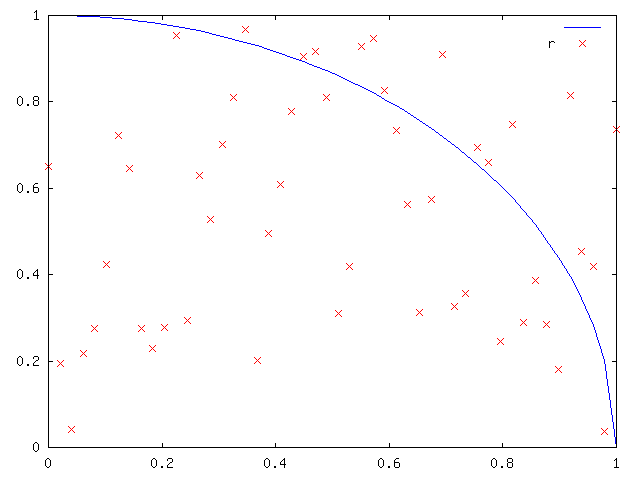
\includegraphics[scale=0.5]{problem_17_1_graph.png}
%\end{center}
% Stop your text

\end{document}
